\documentclass[9pt]{exam} 
\addpoints
\pointsinmargin

\usepackage[fleqn]{amsmath}
\usepackage{amssymb} %standard classy maths symbols
\usepackage[a4paper, margin=1in]{geometry} %makes it easy to specify where to put stuff on the page

\usepackage{tcolorbox} % basic but good package for boxes around text
\tcbset{colback=black!5!white}

\usepackage{tikz} % interval diagrams, sets, etc.

\begin{document}

\textbf{Name:} \dotfill

\

\begin{questions}

\question[3] Let $f(x) = x^2$ and $g(x) = 2x - 1$, with domain $\mathbb{R}$. Find the images of $0$, $4$ and $a + h$ under $f$.
\fillwithdottedlines{20mm}

\question[2] What are the $y$-intercept and gradient of $g$?
\fillwithdottedlines{11mm}

\question[2] Show that the curves $y = f(x)$ and $y=g(x)$ have a single point of intersection and find it.
\fillwithdottedlines{30mm}

\question[2] Sketch the graphs of $f$ and $g$ on these axes.

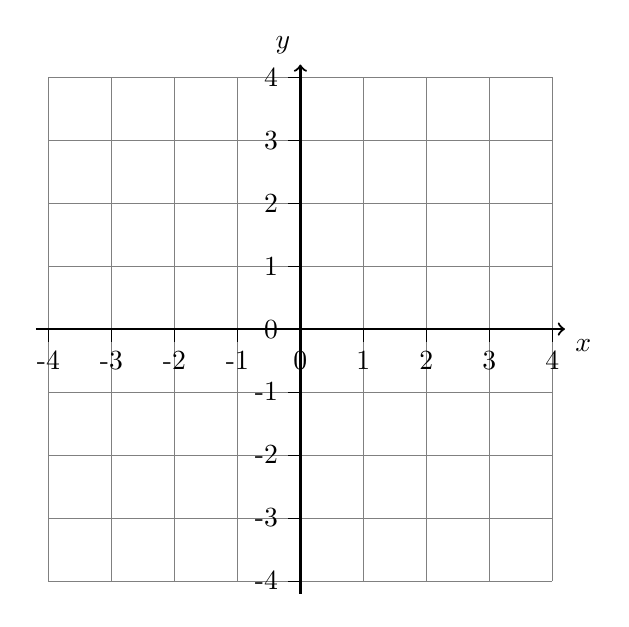
\begin{tikzpicture}[scale=0.8]

% Draw the grid
\draw[step=1cm,gray,very thin] (-4,-4) grid (4,4);

% Draw the x-axis
\draw[thick,->] (-4.2,0) -- (4.2,0) node[anchor=north west] {$x$};

% Draw the y-axis
\draw[thick,->] (0,-4.2) -- (0,4.2) node[anchor=south east] {$y$};

% Add x-axis labels
\foreach \x in {-4,-3,-2,-1,0,1,2,3,4}
    \draw (\x,0) -- (\x,-0.2) node[anchor=north] {\x};

% Add y-axis labels (optional)
\foreach \y in {-4,-3,-2,-1,0,1,2,3,4}
    \draw (0,\y) -- (-0.2,\y) node[anchor=east] {\y};


\end{tikzpicture}

\question[3] Calculate the gradient of $[PQ]$, where $P(2, f(2))$ and $Q(2+h, f(2+h)).$
\fillwithdottedlines{18mm}


\vfill

\question[0] \textbf{Bonus.} Calculate the gradient between $(x, f(x))$ and $(x+h, f(x+h))$. \hfill \emph{Work on the back.}

\end{questions}


\begin{tcolorbox}

\textbf{Name of marker:}

\begin{center}
\gradetable[h][questions]
\end{center}

\end{tcolorbox}


\end{document}